% !TEX root = ../thesis.tex

\chapter{Syntetická časť}

This chapter is focused on the applying of some widespread 2D genome visualization techniques to the SARS-CoV-2 genome. 
Since the topic is extremely complex, only some of existing methods are introduced.
The comprehensive overview of those methods, their analysis and implementation are covered at the corresponding sections.

The second part of this chapter is aimed at the composition of functional but simple software which is capable of visualizing SARS-CoV-2 genome using previously described techniques and libraries.

\section{FASTA, GFF and GBK formats}

To begin with, the understanding of how the genomic data is being stored is the key to the proper visualization.
Generally, the possible solutions for visualization can be divided in two separate categories: those, which use the very genome sequence and those, which use genome annotations \cite{covvisual}.

The first category operates upon the raw DNA (RNA) sequence and is usually used to search for different patterns, tandem repeats, point mutations or to visually compare the genomes of related species.
The raw data either it is DNA (RNA) or aminoacid sequence is usually stored in FASTA format (filename extensions .fasta, .fa, .fna) \cite{fasta}.
The source code below demonstrates the structure of FASTA file containing the SARS-CoV-2 DNA sequence.

\begin{lstlisting}[caption={First 180 nucleotides from SARS-CoV-2 genome sequence in FASTA format. The description line, which begins with '>', contains information about the sequence. Following the initial line is the actual sequence itself in standard one-letter character string.},captionpos=b]
  >NC_045512.2 |Coronavirus 2 isolate Wuhan-Hu-1, complete genome
  ATTAAAGGTTTATACCTTCCCAGGTAACAAACCAACCAACTTTCGATCTCTTGTAGATCT
  GTTCTCTAAACGAACTTTAAAATCTGTGTGGCTGTCACTCGGCTGCATGCTTAGTGCACT
  CACGCAGTATAATTAATAACTAATTACTGTCGTTGACAGGACACGAGTAACTCGTCTATC
\end{lstlisting}


Meanwhile, the second one uses preprocessed and well-studied data \cite{gff}, which is obtained from the raw sequence. 
Genome annotations contain locations of coding regions of genome and therefore they can be useful in fields coherent with genetics, synthesis of proteins, inheritance, etc.
\begin{figure}[!ht]
	\centering
	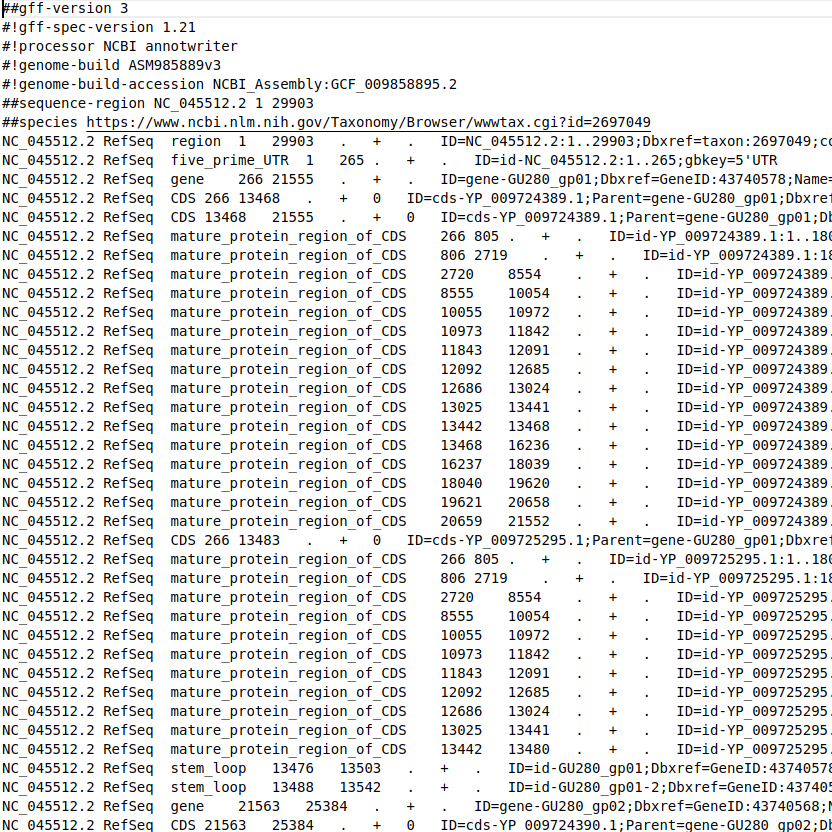
\includegraphics[width=.8\textwidth]{figures/gff3.png}
	\caption{First 45 lines of SARS-CoV-2 genome annotation file. The rightmost part of the annotation is truncated on the image.\label{o:latex_friendly_zone}}
\end{figure}

Each annotation of genome has 9 required fields:
\begin{enumerate}
    \item Sequence ID
    \item Source 
    \begin{itemize}
        \item Describes the algorithm or the procedure that generated this feature. Typically Genescane or Genebank, respectively
    \end{itemize}
    \item Feature Type
    \begin{itemize}
        \item Describes what the feature is (mRNA, domain, exon, etc.)
    \end{itemize}
    \item Feature start
    \item Feature end
    \item Score 
    \begin{itemize}
        \item Values for sequence similarity or predictions
    \end{itemize}
    \item Strand (+ or -)
    \item Phase
    \begin{itemize}
        \item Indicates where the feature begins with reference to the reading frame
    \end{itemize}
    \item Atributes
    \begin{itemize}
        \item A semicolon-separated list of tag-value pairs, providing additional information about each feature
    \end{itemize}
\end{enumerate}
This data is usually stored in GFF (General Feature Format) files. Filename extensions are .gff, .gff2. and .gff3 \cite{gff2}.

Apart from the GFF annotation and FASTA sequence files, the GBK (Genbank format) files are also widely used. 
\begin{figure}[!ht]
	\centering
	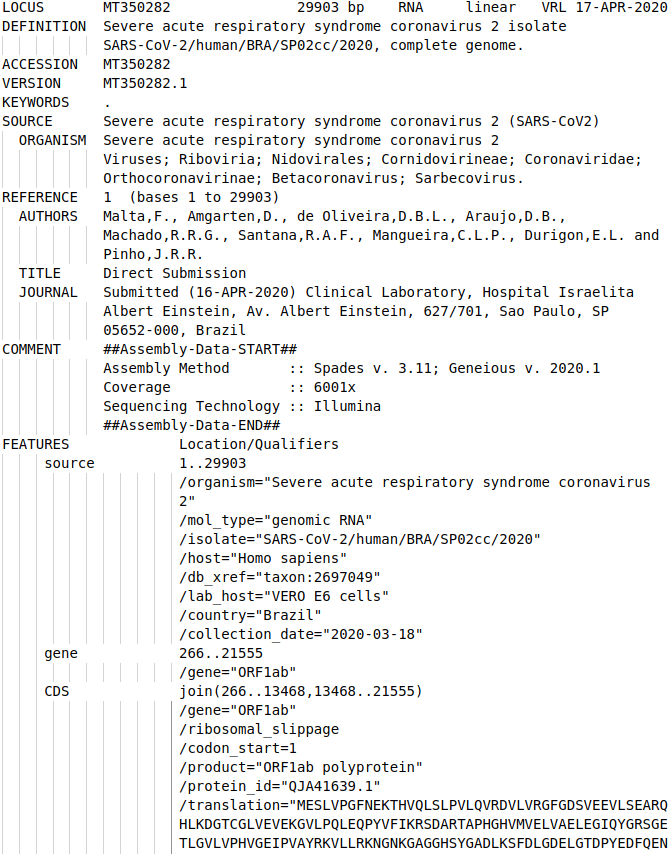
\includegraphics[width=0.7\textwidth]{figures/gbk.png}
	\caption{First 45 lines of contents of GBK file corresponding to SARS-CoV-2 genome\label{o:latex_friendly_zone}}
\end{figure}
The Genbank format allows for the storage of information in addition to a DNA/protein sequence.
The screen grab shows various details, the first section includes the entry’s LOCUS, DEFINITION, ACCESSION and VERSION and denoted by ORIGIN, the final detail is the actual sequence. 
These five elements are the essential parts of the GenBank format.

The non-essential parts of the entry contain what is commonly known as metadata, and can include more detailed information about the organism, cross-references to other databases, and even a list of publications in which this entry is featured in.
The FEATURES part of the entry describes important characteristics of the entry’s sequence such as presence of coding sequences, proteins, etc.

\section{SARS-CoV-2 genome analysis and visualization}
To perform the very analysis, BioPython and DNA features viewer packages will be used.

To visualze the SARS-CoV-2 genome the previously described genome data files are required.
Both the FASTA and GBK files can be obtained at the NCBI webpage (https://www.ncbi.nlm.nih.gov/nuccore/MN908947).

\subsection{Nucleotides distribution and GC-content}

The analysis usually is stared by reading the DNA sequence:
\begin{lstlisting}[language=Python, caption=Python example]
    from Bio.SeqRecord import SeqRecord
    from Bio import SeqIO
    cov19 = SeqIO.read('MN908947.fna', "fasta")
\end{lstlisting}

One of the most essential genomic properties is G-C (or guanine-cytosine content) \cite{gccontent2}.
It is the percentage of nitrogenous bases in a DNA or RNA molecule that are either guanine (G) or cytosine (C).
This measure indicates the proportion of G and C bases out of an implied four total bases, also including adenine and thymine in DNA and adenine and uracil in RNA.

GC-content may be given for a certain fragment of DNA or RNA or for an entire genome. 
When it refers to a fragment, it may denote the GC-content of an individual gene or section of a gene (domain), a group of genes or gene clusters or a non-coding region \cite{gccontent}.

GC-content is usually expressed as a percentage value, but sometimes as a ratio. 
GC-content percentage is calculated as:

    \[\frac{G+C}{A+T+G+C}*100\%\]

The distribution of the nucleotides (A,T,C,G) over the Covid19's DNA can be computed by the attached script.
\begin{lstlisting}[language=Python, caption=The script for computing the distribution of the nucleotides over the SARS-CoV-2 genome.]
    #Count the nucleotides frequency in the DNA
    DNA = SARS_Cov_2_DNA
    nucleotides = {}
    for n in DNA:
        if n in nucleotides:
            nucleotides[n] += 1
        else:
            nucleotides[n] = 1

    #Create a dataframe
    nts = pd.DataFrame(data=nucleotides, 
                                index=[0]).T.reset_index()
    nts = nts.rename(columns={0: 'frequency', 
                                'index': 'nucleotides'})
    nts = nts.sort_values(by=['frequency'], ascending=True)
\end{lstlisting}

The first observation is that the frequency of the nucleotides A (8954) and T (9594)  is higher than the frequency of C (5492) and G (5863). 
Therefore, the GC-content is 37.97\%. 
In comprasion, the GC-content of eukaryotes, such as vertebrates, including humans, can be up to 60\% \cite{gccontent3}.

\begin{figure}[!ht]
	\centering
	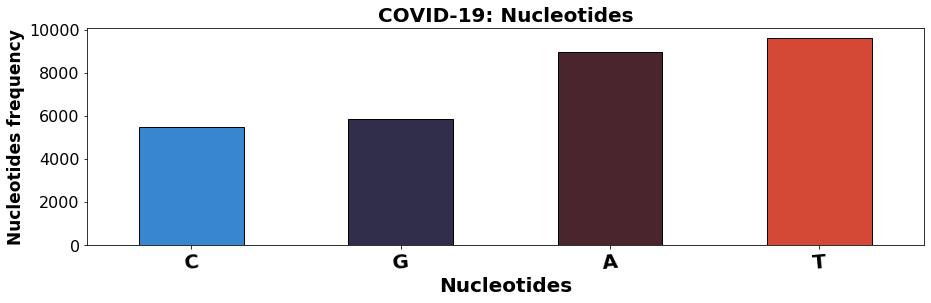
\includegraphics[width=0.9\textwidth]{figures/covidnucleotides.png}
	\caption{Diagram showing the distribution of SARS-CoV-2 nucleotides.\label{o:latex_friendly_zone}}
\end{figure}

\subsection{Gates's method}
The 2D methods are primarily based on the Cartesian coordinate system and the very representation is a set of dots or vectors corresponding to different genome properties;
Gates's method is a typical instance of 2D visualization techniques that operates upon the raw genomic data.
Therefore, the FASTA file is being processed during the visualization.

It is understandable and was chosen as one of methods to implement because it was accidently reinvented by me during the thesis creation.

The four nucleic acid bases are assigned to the four axes of a 2D Cartesian coordinate system.
A given sequence is plotted according to distribution of its bases in the corresponding direction; 
in computations for this note adenine (A) was assigned to the negative x-axis, cytosine (C) to the positive y-axis, guanine (G) to the positive x-axis and thymine (T) to the negative y-axis. 
The weighted average of the x- and y-coordinates of each point of a sequence of length N represents the centre of mass. 
The Euclidean distance between the origin and the centre of mass provides a quantitative graph descriptor, termed as the graph radius (gR). 

This method can be used to search for similarities among related species and for searching patterns in the particular ones.
For instance, after the visualization of SARS-CoV-2 genome sequence using the Gates's method, the sequence of 33 adenine (red) nucleotides is easily distinguishable over the whole genome.
\begin{figure}[!ht]
	\centering
	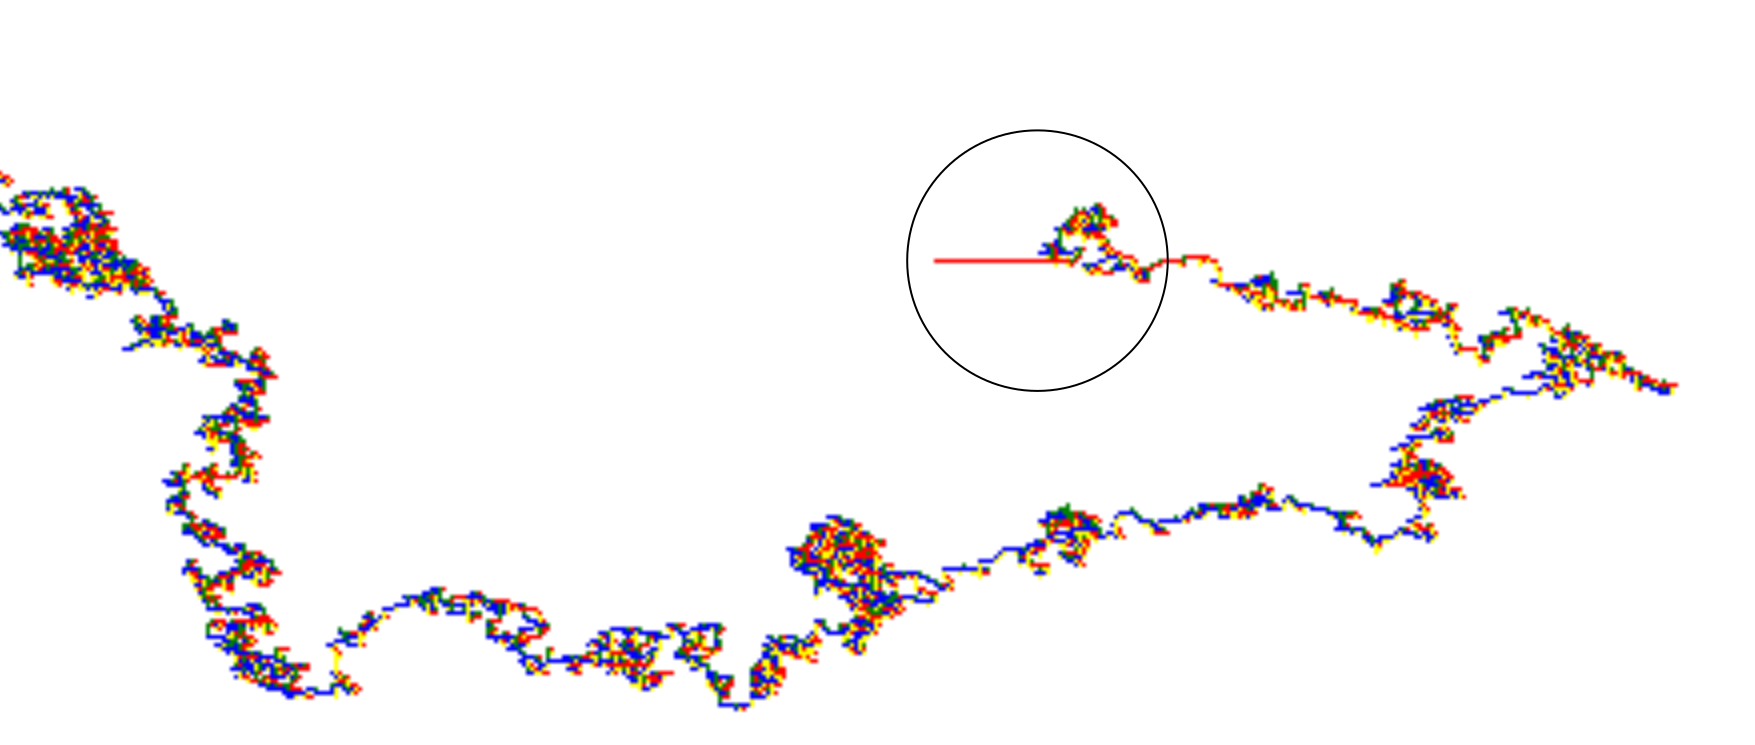
\includegraphics[width=0.6\textwidth]{figures/aaaaa.png}
	\caption{A part of SARS-CoV-2 genome representation using Gates's method. The long sequence of 33 adenine nucleotides is marked at black circle.\label{o:latex_friendly_zone}}
\end{figure}

\begin{figure}[!ht]
	\centering
	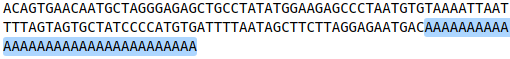
\includegraphics[width=0.7\textwidth]{figures/AAAA.png}
	\caption{Last 143 nucleotides of SARS-CoV-2 virus genome at the FASTA file with the sequenced genome. The long sequence of 33 adenine nucleotides is highlighted.\label{o:latex_friendly_zone}}
\end{figure}

Another instance of finding patterns in DNA sequence using the Gates's method is an attempt of visualization nucleotide sequence of the first chromosome of Encephalitozoon Intestinalis, which is considered to posess the smallest eukaryotic genome.
The sequence can be easily obtained using the NCBI resourse at the following address https://www.ncbi.nlm.nih.gov/nuccore/CP001942.

After the visualization of the mentioned chromosome, the first observation is that both ends of the sequence are almost identical. %%%%cite!!!!!
The only difference, except for point mutations, is that they are composed of complement nucleotides.

\begin{figure}[!ht]
	\centering
	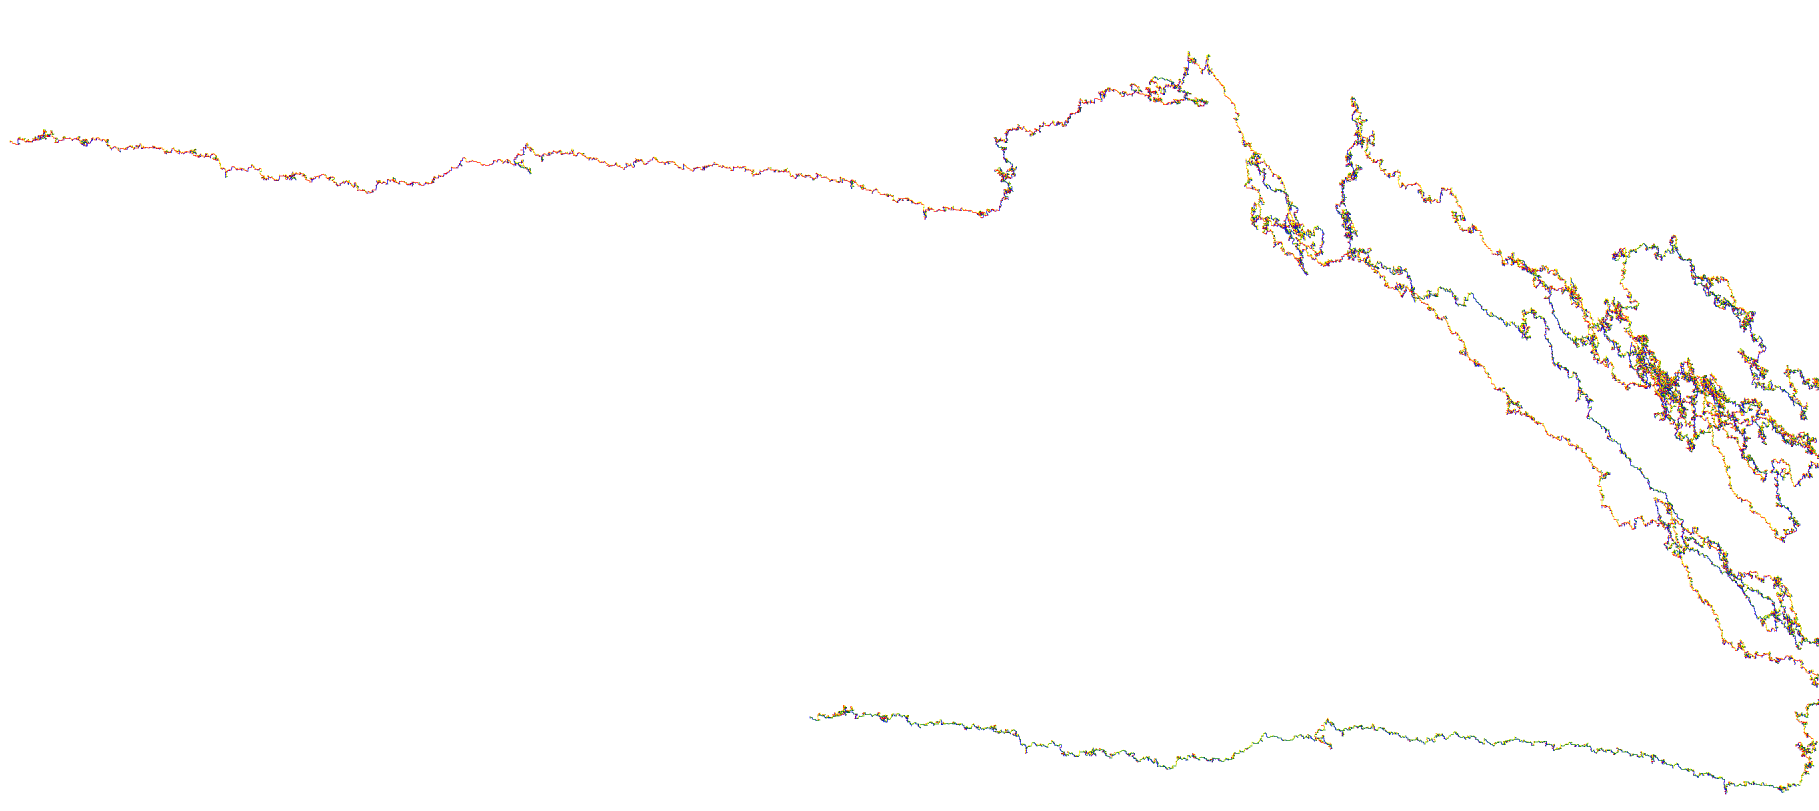
\includegraphics[width=0.7\textwidth]{figures/gateseu.png}
	\caption{Part of the first chromosome visualization of Encephalitozoon Intestinalis. The identical sequences are shown at the middle.\label{o:latex_friendly_zone}}
\end{figure}

The closest relative of modern +ssRNA SARS-CoV-2 virus is SARS-CoV virus, that was the cause of 2004 SARS outbreak.
The comprasion of SARS-CoV and SARS-CoV-2 genome sequences may be considered as the bright example of applying this method.

The very comrasion can be done using the Squiggle, a two-dimensional DNA sequence visualization library \cite{Lee2018}.
\begin{figure}[!ht]
	\centering
	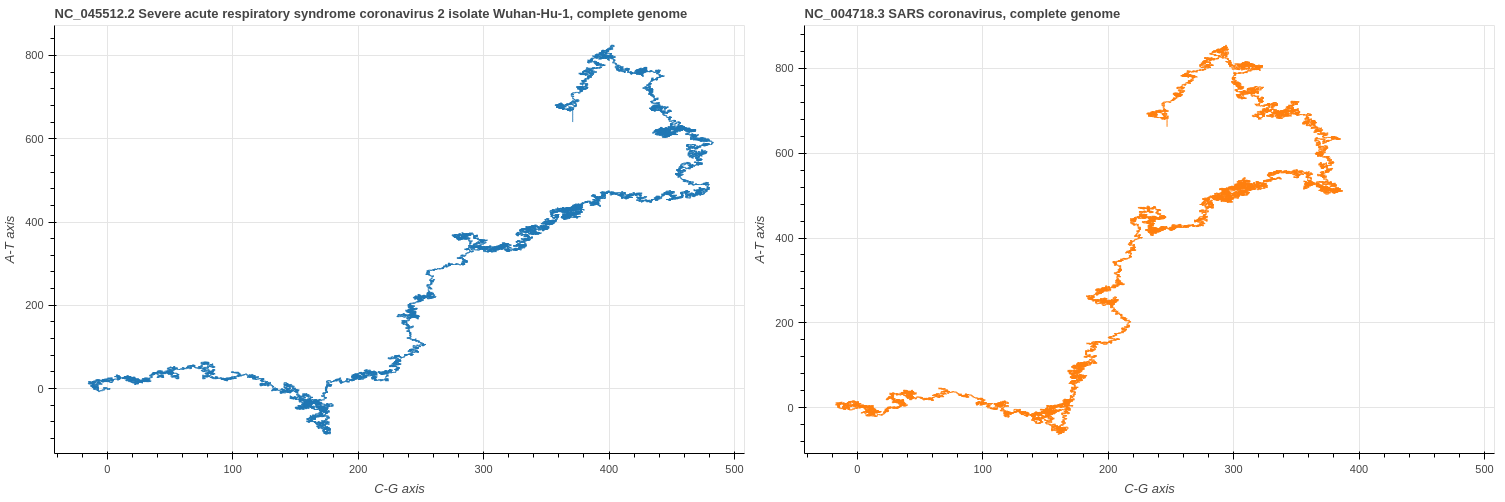
\includegraphics[width=1\textwidth]{figures/comprasion.png}
	\caption{Comprasion of SARS-CoV-2 (from the left) and SARS-CoV (from the right) genomes using Gates's method.\label{o:latex_friendly_zone}}
\end{figure}

As it visible at the provided plot, both of the viruses resemble each other in the terms of the nucleotide sequence \cite{2d}.

After processing the sequences of both viruses with the help of pairwise2 algorithm, the percentage of similarity between them is equal to 83.34\%.

The PairWise algorithm is a variant of the Smith–Waterman algorithm best local alignment algorithm. 
These algorithms all belong to the class known as minimal string edit algorithms. 
It was chosen to compare sequences due to the way he aligns sequences.
The main differences between PairWise and other alignment algorithm is that, besides normal penalties such as Gap Opening Penalty (GOP), Gap Extension Penalty (GEP) and Match, PairWise introduced two new penalties called Frame Opening Penalty (FOP) and Frame Extension Penalty (FEP) \cite{pairwise}.

The very comprasion can be easily done using BioPython library, as demonstrated at the attached code.
\begin{lstlisting}[language=Python, caption=Pairwise2 algorithm using BioPython. COV1.seq and COV2.seq are the DNA sequences of SARS-CoV and SARS-CoV-2 viruses. Two arguments of the very alignment are provided to reduce the alignment comlexity and time.]
    from Bio import pairwise2

    alm = pairwise2.align.globalxx(COV1.seq, COV2.seq,
                 one_alignment_only=True, score_only=True)
    print('Similarity (%):', alm / len(COV2.seq) * 100)
\end{lstlisting}

However, the most important disadvantage of Gates's method is degeneracy, meaning that a visualization is not necessarily unique. 
For example, TGAC is a square (up, right, down, and left), but so is GTCA (right, up, left, down).

\subsection{2D Matrix method}
Another interesting method for DNA visualization, that operates upon the raw DNA squence is 2D matrix method. 
It's aim is to plot whole genome sequence in the square image of predefined size.
Plotting is done from left corner to right corner untill the end of the line, and moving to the left side of the new one afterwards.

Each nucleotide is represented by a pixel (square) of particular color.
\begin{figure}[!ht]
	\centering
	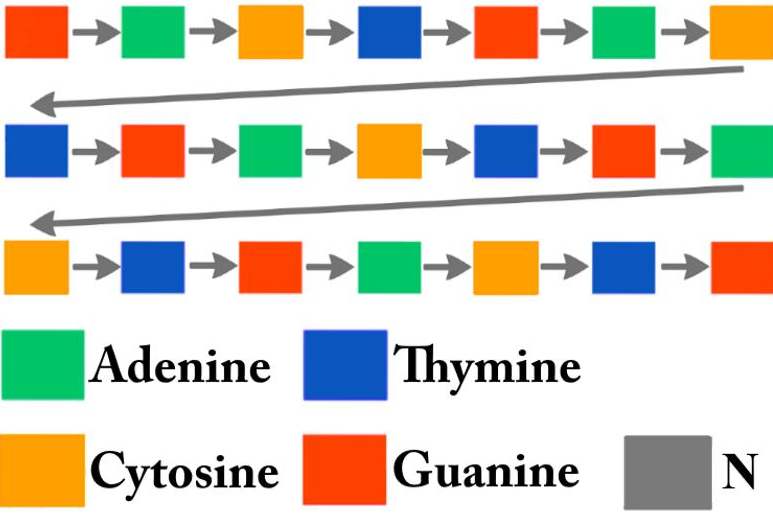
\includegraphics[width=.4\textwidth]{figures/2d.png}
	\caption{The plotting of DNA into the two-dimensional matrix.\label{o:latex_friendly_zone}}
\end{figure}

This method might be useful in finding tandem repeats \cite{fgene} without the detailed examination by a machine since they might be visually detectable.
Moreover, this method plots every genome in the picture of fixed size, that might be used to identify the very sequence uniquely.

\begin{figure}[!ht]
	\centering
	
\includegraphics[width=0.7\textwidth]{figures/matrix.png}
	\caption{Visualization of SARS-CoV-2 genome using the 2D Matrix method. Since the most fluent genome sequence is composed of 29903 nucleotides and the shown matrix contains 29929 positions (173 on each side), the black squares at the right bottom corner represent empty space that was not used for visualization.\label{o:latex_friendly_zone}}
\end{figure}

However, in the case of point mutations, or even significant ones, the difference in the plotted genome might be hardly distinguishable without any machine examination.

\subsection{2D Matrix method improvement}
This thesis suggests new visualization technique which is capable of visualizing each genome uniquely using the hash-function \cite{hash}, which might be a solution to the menioned above disadvantage.

The main idea of the visualization technique is a recursive algorithm that partitions the image into smaller parts coloring each one depending on the pevious one.
This prevents the random noise that might appear by breaking it into tiny bits and coloring each one independently. 
Instead, there are larger regions which maintain some continuity even though their constituent parts diverge.

The recursive algorithm is composed of three functions: 
\begin{itemize}
    \item Function, which achieves a hash of the nucleotide sequence using sha256 algorithm.
    \item Function, which recursively partitions the initial empty image in 1/8 parts.
    It is done recursively 8 times to each of the initial partitions. 
    \item Function, which colors each partition according to the hash and inserts each partition above the bigger one.
    The opacity parameter that is computed of each partition size and used to prevent the overlapping between colors of smaller partitions and bigger ones (that are colored before).
\end{itemize}

Listing 2.5 demonstrates the console output during the creation of image which is 512x512 pixels in size.
The width and heigh values represent the sizes of partitioned images that are being colored, and the opacity value shows the opacity during each partition overlaps.
The images generated to illustrate this method were using the opacity equation defined as:\\
\[opacity = 256 * (level / 2) / 2 ^ {(level - 1)}\]
where level represents the current depth of recursion.
However, this equation can be changed to intoduce another coloring schemes.

\begin{lstlisting}[caption=Console output prodused during the visualization using the improved 2D Matrix method.]
    seed: 223dd4d5c80b98e69f9f8536afa54b...
    width, height: 256.0, 256.0
    opacity: 50%
    width, height: 128.0, 64.0
    opacity: 37%
    width, height: 32.0, 32.0
    opacity: 25%
    width, height: 16.0, 8.0
    opacity: 15%
    width, height: 4.0, 4.0
    opacity: 9%
    width, height: 2.0, 1.0
    opacity: 5%
\end{lstlisting}

As it is visible on the figure 2.10, this method lets different genomes be easily distinguished with the naked eye.

\begin{figure}[!ht]
	\centering
	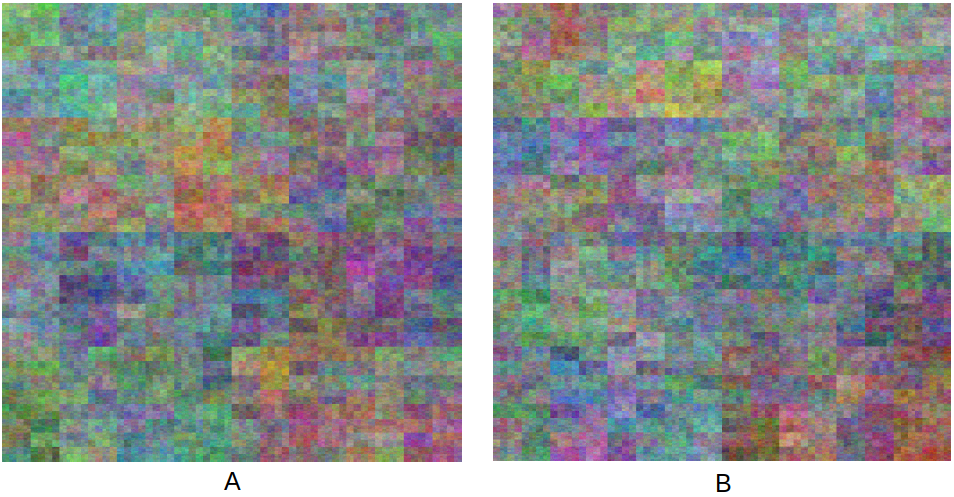
\includegraphics[width=1\textwidth]{figures/2dim.png}
	\caption{Visualization of original SARS-CoV-2 genome [A] and the same genome with a point mutation [B] at the second nucleotide (T changed on G) using the improved 2D Matrix method.\label{o:latex_friendly_zone}}
\end{figure}

Because of the recursive nature of the algorithm, the image can be generated at smaller or larger sizes and maintain the same level of detail.

However, among the main disadvantages are the small practical usage and a limit regarding the size of a genome.
Currently, the method suports the visualization of genomes that are less than 262145 nucleotides long.

\subsection{Aminoacids retrieval}

For the next visualization the raw DNA sequence must be converted to the sequence of aminoacids.
There are 61 codons (trinucleotides) for 20 amino acids, and each of them is "read" to specify a certain amino acid out of the 20 commonly found in proteins.
Each aminoacid can be written as a letter of latin alphabet.
Therefore, the sequence of aminoacids is represented by the sequence of letters A-V. 

One codon, AUG, specifies the amino acid methionine and also acts as a start codon to signal the start of protein construction.
There are three more codons that do not specify amino acids: UAA, UAG, and UGA, tell the cell when a polypeptide is complete. 
All together, this collection of codon-amino acid relationships is called the genetic code, because it lets cells “decode” an mRNA into a chain of amino acids.

Before converting the DNA sequence into the aminoacid one, firstly, has to be transcribed into the mRNA molecule \cite{rnaseqexp} with the help of transcribe() function.
Luckily, with the translate() function, BioPython does translate the mRNA to amino acids chains. 
Chains are separated with a * which is the stop codon (UAA, UAG and UGA).

\begin{lstlisting}[language=Python, caption=Transcription and translation using BioPython]
    cov_DNA = covid19.seq
    cov_mRNA = covid_DNA.transcribe()
    cov_aa = covid_mRNA.translate()
\end{lstlisting}

SARS-CoV-2 genome contains 9967 aminoacids separated with stop codons * or, in other words, 775 amino acid chains.
It's worth to mention that not all the amino acids sequences are proteins. 
Only the sequences with more than 20 amino acids code for functional proteins. 
The short amino acid sequences are oligopeptides and have other functionalities. 
The next step is to filter obtained sequences in such a way, that only long ones will remain to focus only on proteins.

After the removal of short proteins, only 5 of remaining ones satisfy the length condition (source code 2.6) and are provided at the table 2.1 .

The easiest way to verify results is to find the protein sequences already available in the databases that are the most similar to obtained protein sequences. 
The BLAST search was used for these purposes.

BLAST (basic local alignment search tool) is an algorithm and program for comparing primary biological sequence information, such as the amino-acid sequences of proteins or the nucleotides of DNA and/or RNA sequences. 
A BLAST search enables a researcher to compare a subject protein or nucleotide sequence (called a query) with a library or database of sequences, and identify library sequences that resemble the query sequence above a certain threshold.

\begin{lstlisting}[language=Python, caption=Filtering aminoacid sequences and storing them in a dataframe]
    Proteins = covid_aa.split('*')

    #Remove porteins with less than than 50 amino acids
    for i in Proteins[:]:
        if len(i) < 50:
            Proteins.remove(i)
    #Store the protein sequences in a pandas dataframe

    proteins=pd.DataFrame(Proteins)
    proteins['amino acid sequence'] = proteinas[0].apply(str)
    proteins['Protein length'] = proteinas[0].apply(len)
    proteins.rename(columns={0: "sequence"}, inplace=True)
    pro=proteins.drop('sequence', axis=1)
    pro=pro.sort_values(by=['Protein length'], ascending=False)
\end{lstlisting}

\begin{table}[]
    \caption{Obtained protein sequences of SARS-CoV-2 genome that are composed of more than 50 aminoacids.}\label{t:1}
	\smallskip
	\centering
    
    \begin{tabular}{|l|l|c|}
    \hline
    \textbf{ } & \textbf{Aminoacid sequence}                                                     & \multicolumn{1}{l|}{\textbf{Protein length}} \\ \hline
    \textbf{1} & CTIVFKRVCGVSAARLTPCGTGTSTDVVYRAFDIYND... & 2701                                         \\ \hline
    \textbf{2} & ASAQRSQITLHINELMDLFMRIFTIGTVTLKQGEIKD... & 290                                          \\ \hline
    \textbf{3} & TNMKIILFLALITLATCELYHYQECVRGTTVLLKEPC... & 123                                          \\ \hline
    \textbf{4} & AQADEYELMYSFVSEETGTLIVNSVLLFLAFVVFLLV... & 83                                           \\ \hline
    \textbf{5} & QQMFHLVDFQVTIAEILLIIMRTFKVSIWNLDYIINL... & 63                                           \\ \hline
    \end{tabular}
\end{table}

After searching for the 83 aminoacid chain using BLAST, the results have shown that it has 100\% similarity with Envelope small membrane protein that belongs to SARS-CoV-2 genome.
The results of performed BLAST searches for other obtained proteins are attached at the table 2.2 .
It is worth mentioning, that the highest similarities were found among other coronavirus species.

\begin{table}[]
    \caption{Results of comprasion between obtained protein sequences of SARS-CoV-2 using BLAST.}\label{t:1}
	\smallskip
	\centering
    \begin{tabular}{|c|c|c|c|c|c|}
        \hline
        \multicolumn{1}{|l|}{}             & \multicolumn{1}{l|}{\textbf{\begin{tabular}[c]{@{}l@{}}Protein \\ length\end{tabular}}} & \multicolumn{1}{l|}{\textbf{DB:ID}} & \multicolumn{1}{l|}{\textbf{Organism}}                                                                  & \multicolumn{1}{l|}{\textbf{Protein}}                                                                  & \multicolumn{1}{l|}{\textbf{Match}} \\ \hline
        \multicolumn{1}{|c|}{\textbf{1}} & \multicolumn{1}{c|}{2701}                                                              & \multicolumn{1}{c|}{P0C6X7}        & \multicolumn{1}{c|}{\begin{tabular}[c]{@{}c@{}}Replicase \\ polyprotein \\ 1ab\end{tabular}}           & \multicolumn{1}{c|}{\begin{tabular}[c]{@{}c@{}}Replicase \\ polyprotein \\ 1ab\end{tabular}}          & \multicolumn{1}{c|}{96\%}           \\ \hline
        \multicolumn{1}{|c|}{\textbf{2}} & \multicolumn{1}{c|}{290}                                                               & \multicolumn{1}{c|}{Q0Q474}        & \multicolumn{1}{c|}{\begin{tabular}[c]{@{}c@{}}Bat \\ coronavirus \\ 279/2005 \\ (BtCoV)\end{tabular}} & \multicolumn{1}{c|}{Protein 3}                                                                        & \multicolumn{1}{c|}{75\%}           \\ \hline
        \multicolumn{1}{|c|}{\textbf{3}} & \multicolumn{1}{c|}{123}                                                               & \multicolumn{1}{c|}{Q3I5J0}        & \multicolumn{1}{c|}{\begin{tabular}[c]{@{}c@{}}Bat \\ coronavirus \\ Rp3/2004\end{tabular}}            & \multicolumn{1}{c|}{Protein 7a}                                                                       & \multicolumn{1}{c|}{89\%}           \\ \hline
        \multicolumn{1}{|c|}{\textbf{4}} & \multicolumn{1}{c|}{83}                                                                & \multicolumn{1}{c|}{P0DTC4}        & \multicolumn{1}{c|}{\begin{tabular}[c]{@{}c@{}}Human SARS \\ coronavirus \\ (SARS-CoV-2)\end{tabular}} & \multicolumn{1}{c|}{\begin{tabular}[c]{@{}c@{}}Envelope \\ small \\ membrane \\ protein\end{tabular}} & \multicolumn{1}{c|}{100\%}          \\ \hline
        \multicolumn{1}{|c|}{\textbf{5}} & \multicolumn{1}{c|}{63}                                                                & \multicolumn{1}{c|}{Q3I5J1}        & \multicolumn{1}{c|}{\begin{tabular}[c]{@{}c@{}}Bat \\ coronavirus \\ Rp3/2004\end{tabular}}            & \multicolumn{1}{c|}{\begin{tabular}[c]{@{}c@{}}Non-\\ structural \\ protein 6\end{tabular}}           & \multicolumn{1}{c|}{69\%}           \\ \hline
        \end{tabular}
\end{table}

\subsection{ORF identification and visualization}
The next visualization operates upon the preprocessed data stored at the GenBank annotation file.
As it was mentioned at the first chapter of this thesis, ORF scanning is not a full proof of finding gene locations since not every ORF is a gene beginning.
However, the longer ORF is, the likely it is a part of gene. \cite{orf}

The identification of coding sequences (CDS) is an important step in the functional annotation of genes. 
A typical CDS starts with ATG and ends with a stop codon.
CDS is a sequence of nucleotides that corresponds with the sequence of amino acids in a protein. 
Therefore, the amino acids analysis and retrieval (done in section 2.2.5) was necessary to identify coding regions of genome.
The SARS-CoV-2 genome encodes as far as 50 non-structural, structural, and accessory proteins.

The source code 2.7 is an output a script for visualization that finds the ORFs in the SARS-CoV-2 genome using genome annotation file. 
The minimum protein length is set to 200 amino acids to retrieve only long ORFs.

\begin{lstlisting}[caption=Positions of SARS-CoV-2 genome CDSs]
    PKGKMESLVPGFNEKTH...FAV - length 4409, strand 1, 253:13483
    CTIVFKRVCGVSAARLT...VNN - length 2701, strand 1, 13449:21555
    LEKTTELLFLVMFLLTT...HYT - length 1293, strand 1, 21502:25384
    ASAQRSQITLHINELMD...VPL - length 290, strand 1, 25347:26220
    SSGLNELNIILVFLFGT...LVQ - length 243, strand 1, 26459:27191
    RSCCFRFHLNEQTKMSD...TQA - length 433, strand 1, 28231:29533
\end{lstlisting}

The Covid-19 genome has 6 ORFs with more than 200 amino acids. Figure 2.11 demonstrates all the ORFs and CDSs retrieved from the SARS-CoV-2 genome using BioPython.

\begin{figure}[!ht]
	\centering
	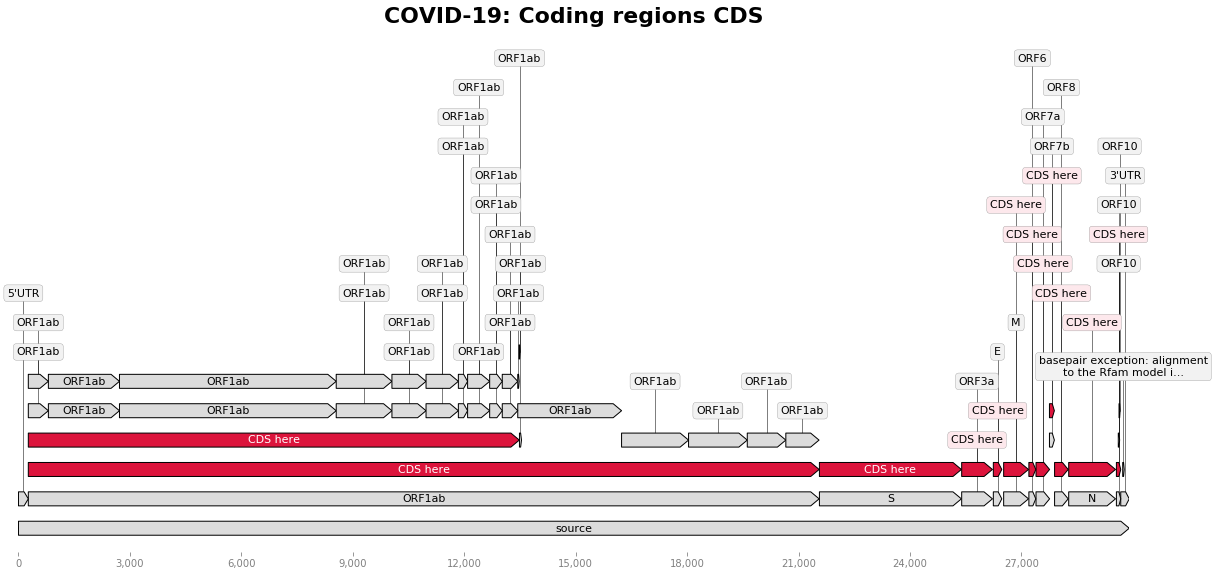
\includegraphics[width=1\textwidth]{figures/cds.png}
	\caption{Coding regions of SARS-CoV-2 genome are highlighted in red among other ORFs. They include the ORF1ab, ORF3a, S protein, M protein and N protein. The visualization is done using BioPython\label{o:latex_friendly_zone}}
\end{figure}

The results of comparing obtained sequences to the existing ones are performed using BLAST and listed at the table 2.3 .

\begin{table}[]
    \caption{BLAST search results for SARS-CoV-2 ORFs.}\label{t:1}
	\smallskip
	\centering

    \begin{tabular}{|c|c|c|c|c|c|}
    \hline
               & \textbf{\begin{tabular}[c]{@{}c@{}}ORF\\ length\end{tabular}} & \textbf{DB:ID} & \textbf{Protein}                                                        & \textbf{Organism}                                                                 & \textbf{Match} \\ \hline
    \textbf{1} & 4409                                                          & P0C6U8         & \begin{tabular}[c]{@{}c@{}}Replicase\\ polyprotein \\ 1a\end{tabular}   & \begin{tabular}[c]{@{}c@{}}Human \\ SARS\\ coronavirus \\ (SARS-CoV)\end{tabular} & 80\%           \\ \hline
    \textbf{2} & 2701                                                          & P0C6X7         & \begin{tabular}[c]{@{}c@{}}Replicase \\ polyprotein \\ 1ab\end{tabular} & \begin{tabular}[c]{@{}c@{}}Human \\ SARS\\ coronavirus \\ (SARS-CoV)\end{tabular} & 96\%           \\ \hline
    \textbf{3} & 1293                                                          & P59594         & \begin{tabular}[c]{@{}c@{}}Spike\\ glycoprotein\end{tabular}            & \begin{tabular}[c]{@{}c@{}}Human \\ SARS\\ coronavirus \\ (SARS-CoV)\end{tabular} & 76\%           \\ \hline
    \textbf{4} & 290                                                           & Q0Q474         & Protein 3                                                               & \begin{tabular}[c]{@{}c@{}}Bat\\ coronavirus\\ Rp3/2004\end{tabular}              & 95\%           \\ \hline
    \textbf{5} & 243                                                           & Q0Q472         & \begin{tabular}[c]{@{}c@{}}Membrane\\ protein\end{tabular}              & \begin{tabular}[c]{@{}c@{}}Bat\\ coronavirus\\ Rp3/2004\end{tabular}              & 92\%           \\ \hline
    \textbf{6} & 433                                                           & P59595         & \begin{tabular}[c]{@{}c@{}}Nucleoprotein\\ N\end{tabular}               & \begin{tabular}[c]{@{}c@{}}Human \\ SARS\\ coronavirus \\ (SARS-CoV)\end{tabular} & 91\%           \\ \hline
    \end{tabular}
\end{table}

\section{Software composition}
The software developed during this thesis appears to be a collection of scripts used to visualize SARS-CoV-2 genome in previously described methods.
In general, unlike the web based genome browsers where the computations are done at the server side, the suggested software represent a simple stand-alone console application.
No significant computations are being done and, therefore, the application do not satisfying of demanding system requirements.

The software is written mainly using the BioPython package in Python 3.8 .
All the packages that are required are mentioned at the project documentation.

The main idea of a program is to let the user choose which information regarding the virus genome he wants to visualize.
It consists of 9 modules which have own role at the very process of visualization:
\begin{enumerate}
    \item \textbf{Main Module} is the core of the program. It is responsible for providing user with navigation within the program.
    It handles console input and output, suggests available methods of visualiation and retrieves details required for their performance.
    \item \textbf{Sequence Collector} is responsible for downloading all the required sequences and annotation files from NCBI database.
    \item \textbf{Statistics Generator} obtains the statistical data such as GC-content and nucleotide / aminoacid distribution.
    User is able to choose the region of genome which statistics should be collected and to choose whether he wants his data to be saved into particular file.
    \item \textbf{Gates Visualization} performs a visualization using the Gates's method into a .png file.
    User is able to adjust color dependencies.
    \item \textbf{2D Matrix} module plotes the selected genome into a 2D matrix into a .png file.
    The size of an output picture is computed automatically.
    \item \textbf{2D IMatrix} module plotes a genome into a 2D matrix of the selected size using the hash function algorithm into a .png file.
    The bigger size, the more RAM memory is needed.
    \item \textbf{Protein Plotter} generates protein sequences of a genome according to the nucleotide sequence.
    User is able to remove those, that do not satisfy length conditions and is able to chose whether to print the results or to store them into a .csv file.
    \item \textbf{ORF Plotter} generates an image of SARS-CoV-2 ORFs and GC-content ratio within the genome.
    \item \textbf{Comprasion} module performs a comprasion of selected genomes.
    The similarity percentage is obtained using the pairwise2 algorithm.
\end{enumerate}

Modules do not able to interact with each other, but every of them can be called from the main one.

Each of the modules is described at the documentation and accompanied with the input and output examples.
Moreover, every module contains different run-time tests which prevent unexpected program behaviour.

At the moment all the modules, except for ORF Plotter, support processing of various genomes.
However, it is not recommended to use Protein Plotter with genomes that contain complex intron-exon structures due to their complexity.
In such a case, results might differ significantly from the real characteristics of genome.